\chapter[Cenários de Teste]{Cenários de Teste}
\label{sec:cenarios_teste}
O principal objetivo dos cenários de teste é apoiar a observação e análise sistemática da técnica de auto-localização utilizada durante o trabalho, assim como as diferentes configurações do ambiente e
do filtro utilizado.

Após a realização de todos os cenários de teste propostos, deve-se chegar a uma conclusão referente a viabilidade da utilização da técnica do Filtro de Partículas em um contexto simplificado da robótica.

Os cenários de teste consistem em 10 situações onde a solução foi analisada, variando entre elas o ambiente e a configuração do filtro. Buscando
analisar a exatidão da auto-localização obtida em cada contexto, reiterando que o objetivo da pesquisa é analisar a viabilidade da utilização
de uma técnica de SLAM em um contexto simplificado.

O Filtro de Partículas é uma das duas principais técnicas que buscam solucionar o problema
de SLAM, por este motivo, os cenários de teste desta pesquisa buscam analisar o Filtro de Partículas sendo executado no contexto da Robótica
Educacional, o que viabilizaria, em parte, a aplicação da solução de SLAM no contexto simplificado.

Os dados obtidos a partir de cada cenário de teste está organizado de acordo com a Tabela \ref{tab:org_dados}.

\begin{table}[H]
  \centering
  \caption{Organização dos Dados}
  \label{tab:org_dados}
  \begin{tabular}{|c|c|c|c|}
  \hline
  \textbf{Exemplo} & \textbf{Partículas} & \textbf{Movimentos} & \textbf{Erro} \\ \hline
  \end{tabular}
\end{table}

Onde, \textbf{Exemplo} faz referência ao ciclo de teste. Cada cenário foi testado 5 (cinco) vezes, buscando obter a média como resultado
final do cenário. \textbf{Partículas} informa a quantidade de partículas utilizada durante este teste, \textbf{Movimentos} apresenta
o número de movimentos aleatórios que foram necessários para obtenção da localizaão e o \textbf{Erro} informando qual o erro obtido no teste, ou seja,
qual a distância, em centímetros (cm), entre a posição obtida e a posição real do robô.

\subsection{Cenário de Teste 1}

Durante este cenário de teste, o ambiente utilizado foi o apresentado na Figura \ref{img:map1}, onde todos os
valores se encontram em centímetros (cm), e os resultados obtidos com o cenários estão dispostos na Tabela \ref{tab:cen1}.

\begin{figure}[H]
	\centering
	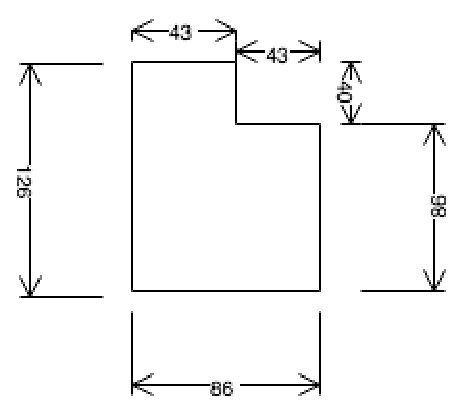
\includegraphics[scale=1.3]{figuras/map1.eps}
	\caption[Primeiro Cenário de Teste]{Mapa utilizado durante primeiro cenário de teste.}
	\label{img:map1}
\end{figure}

\begin{table}[H]
  \centering
  \caption{Resultados obtidos - Cenário 1}
  \label{tab:cen1}
  \begin{tabular}{|c|c|c|c|}
  \hline
  \textbf{Exemplo} & \textbf{Partículas} & \textbf{Movimentos} & \textbf{Erro} \\ \hline
  1                & x                   & y                   & z             \\ \hline
  \end{tabular}
\end{table}
